\documentclass[a4paper,14pt]{extarticle}
\usepackage{geometry}
\geometry{top=20mm,bottom=20mm,left=30mm,right=10mm} % поля по требованиям оформления
\usepackage{fontspec}
\usepackage[russian]{babel}
% \setmainfont{Liberation Serif}
\setmainfont{Times New Roman}
\usepackage{setspace}
\usepackage{indentfirst}
\usepackage{titlesec}

\usepackage{amsmath}
\usepackage{caption}
\usepackage{graphicx}
\usepackage{float}
\usepackage{tikz}
\usetikzlibrary{arrows.meta,positioning}
\usepackage{url}
\usepackage{array}
\usepackage{tocloft}
\usepackage[hidelinks]{hyperref}

\setcounter{tocdepth}{3}
\onehalfspacing
\setlength{\parindent}{1.25cm}
\pagestyle{plain}
\renewcommand{\cftsecleader}{\cftdotfill{\cftdotsep}}
\renewcommand{\cftsubsecleader}{\cftdotfill{\cftdotsep}}
\renewcommand{\cftsubsubsecleader}{\cftdotfill{\cftdotsep}}

\titleformat{\section}{\centering\normalfont\bfseries}{\thesection}{1em}{\MakeUppercase}
\titleformat{name=\section,numberless}{\centering\normalfont\bfseries}{}{0pt}{\MakeUppercase}
\titleformat{\subsection}{\centering\normalfont\bfseries}{\thesubsection}{1em}{\MakeUppercase}
\titleformat{\subsubsection}{\centering\normalfont\bfseries}{\thesubsubsection}{1em}{\MakeUppercase}
\titlespacing*{\section}{0pt}{0pt}{1.5\baselineskip}
\titlespacing*{\subsection}{0pt}{1.5\baselineskip}{1.5\baselineskip}
\titlespacing*{\subsubsection}{0pt}{1.5\baselineskip}{1.5\baselineskip}
\newcommand{\sectionbreak}{\clearpage}

\begin{document}

\begin{titlepage}
    \centering
    {МИНОБРНАУКИ РОССИИ\par}
    \vspace{0.5em}
    {САНКТ-ПЕТЕРБУРГСКИЙ ГОСУДАРСТВЕННЫЙ\par}
    {ЭЛЕКТРОТЕХНИЧЕСКИЙ УНИВЕРСИТЕТ\par}
    {«ЛЭТИ» ИМ. В.И. УЛЬЯНОВА (ЛЕНИНА)\par}
    \vspace{1em}
    {Кафедра информационных систем\par}

    \vspace{6em}

    {\textbf{КУРСОВАЯ РАБОТА}\par}
    \vspace{0.8em}
    {по дисциплине «Методы и средства проектирования информационных систем»\par}
    \vspace{0.8em}
    {Тема: «Разработка приложения для работы со справочником»\par} % впишите тему или оставьте линию
    %\vspace{0.8em}
    %{\large Вариант №\par} % впишите тему или оставьте линию

    \vfill % «утопить» нижний блок к низу страницы

    \begin{flushleft}
    \begin{tabular*}{\linewidth}{@{}l@{\extracolsep{\fill}}c@{\extracolsep{\fill}}r@{}}
    Студент гр. 3376  & \rule{4cm}{0.4pt} & Михайлов Н.Ф.\\[0.5em]
    Студентка гр. 3376 & \rule{4cm}{0.4pt} & Дегтярева М. И.\\[0.5em]
    Студент гр. 3376  & \rule{4cm}{0.4pt} & Константинов Р. И.\\[0.5em]
    Преподаватель     & \rule{4cm}{0.4pt} & Дюков Н.В.
    \end{tabular*}
    \end{flushleft}

    \vspace{3em}

    Санкт-Петербург\par
    2026
\end{titlepage}

\newpage
\section*{Задание на курсовую работу}
\addcontentsline{toc}{section}{Задание на курсовую работу}

\noindent Студент Михайлов Н.Ф.\\
Студентка Дегтярева М. И.\\
Студент Константинов Р. И.\\
Группа 3376\\
Тема работы: Разработка приложения для работы со справочником

\vspace{1em}
\noindent\textbf{Исходные данные:}

Создать приложение для работы со справочником изделий, которое хранит классификатор, товары, параметры, перечисления и единицы измерения в базе данных, предоставляет доступ к данным посредством API сервера и содержит пользовательский web-интерфейс для просмотра, фильтрации и управления данными справочника.

\vspace{1em}
\noindent\textbf{Содержание пояснительной записки:}

«Аннотация», «Содержание», «Введение», «Анализ предметной области», «Разработка объектной модели этапа проектирования», «Разработка модели хранения», «Разработка базы данных», «Разработка основных процедур», «Разработка пользовательского интерфейса», «Результаты тестирования», «Заключение», «Список использованных источников», «Приложение».

\vspace{1em}
\noindent\textbf{Предполагаемый объем пояснительной записки:}

Не менее 25 страниц.

\vspace{1em}
\noindent Дата выдачи задания: 01.04.2026\\
Дата сдачи реферата: 28.05.2026\\
Дата защиты реферата: 28.05.2026

\vspace{3em}

\noindent
\begin{tabular}{@{}p{4cm}c>{\raggedleft\arraybackslash}p{5cm}@{}}
Студент(ка)  & \rule{4cm}{0.4pt} & Михайлов Н.Ф.\\[0.5em]
Студент(ка)  & \rule{4cm}{0.4pt} & Дегтярева М. И.\\[0.5em]
Студент(ка)  & \rule{4cm}{0.4pt} & Константинов Р. И.\\[0.5em]
Преподаватель & \rule{4cm}{0.4pt} & Дюков Н.В.
\end{tabular}

\newpage
\section*{Аннотация}
\addcontentsline{toc}{section}{Аннотация}

В работе описана разработка web-приложения для справочника электронных комплектующих. Приложение хранит категории, товары, характеристики, параметры, перечисления и единицы измерения в PostgreSQL, а доступ к данным организован через API на FastAPI. Для пользователя сделана витрина с фильтрами и корзиной, для администрирования предусмотрены формы управления категориями и товарами. В пояснительной записке приведены анализ предметной области, структура базы данных, архитектура приложения, описание интерфейса и результаты проверки основных сценариев.

\vspace{1em}
\begin{center}
\textbf{SUMMARY}
\end{center}

This paper describes the development of a web application for an electronic components catalog.
The application stores categories, products, specifications, \\ parameters, enumerations and measurement units in PostgreSQL, and provides access to the data through a FastAPI-based API. The user interface includes a product showcase with filters and a shopping cart. Administrative forms are provided for managing categories and products. The explanatory note includes the domain analysis, database structure, application architecture, interface description and the results of testing the main scenarios.

\newpage
\tableofcontents

\newpage
\section{Введение}

В данной курсовой работе разрабатывается web-приложение для работы со справочником электронных комплектующих.
Предметная область выбрана на примере каталога электроники: процессоров, видеокарт, материнских плат и других товаров.

Цель работы --- спроектировать и разработать приложение, которое позволяет хранить классификатор изделий в базе данных, управлять товарами и их параметрами через API, а также работать с этими данными через пользовательский web-интерфейс.

Для достижения цели необходимо решить следующие задачи:
\begin{itemize}
    \item проанализировать предметную область и определить основные сценарии работы пользователей;
    \item разработать модель категорий, товаров, характеристик, параметров, перечислений и единиц измерения;
    \item реализовать хранение данных в PostgreSQL;
    \item разработать REST API для управления справочником;
    \item создать web-интерфейс для просмотра каталога, фильтрации товаров и работы с корзиной;
    \item предусмотреть административные формы для добавления и редактирования основных сущностей;
    \item проверить работу приложения на основных сценариях.
\end{itemize}

Практическая значимость работы состоит в том, что пользователь получает доступ к справочнику через браузер без установки дополнительного программного обеспечения. Администратор может изменять структуру каталога и наполнение справочника, а пользователь витрины -- искать товары по категории, цене, наличию и характеристикам.

\section{Основная часть}

\subsection{Анализ предметной области}

\subsubsection{Цели и задачи}

Цель ИС -- автоматизация ведения справочника электронных комплектующих и предоставление удобного доступа к данным через web-интерфейс и API. Система должна хранить классификатор изделий, товары, характеристики, параметры, перечисления и единицы измерения в базе данных. Пользователь работает со справочником через витрину, а администратор управляет структурой и наполнением каталога.

Требования к контенту и функционалу:

Администратор может:
\begin{itemize}
    \item создавать, редактировать и удалять категории справочника;
    \item добавлять товары электронных комплектующих и изменять их основные данные;
    \item задавать характеристики товаров, в том числе значения с единицами измерения;
    \item создавать перечисления и наполнять их значениями, например сокетами, форм-факторами или типами памяти;
    \item создавать параметры разных типов и привязывать их к категориям товаров;
    \item задавать ограничения для числовых параметров;
    \item использовать наследование параметров от родительских категорий;
    \item проверять работу справочника через API и административные формы интерфейса.
\end{itemize}

Пользователь может:
\begin{itemize}
    \item просматривать каталог электронных комплектующих;
    \item выбирать категорию товаров;
    \item искать товары по названию и описанию;
    \item фильтровать товары по цене, наличию и характеристикам;
    \item просматривать краткую информацию о товаре и его параметрах;
    \item добавлять товары в корзину, изменять количество и удалять позиции из корзины;
    \item пользоваться системой без доступа к изменению справочных данных.
\end{itemize}

\subsubsection{Описание пользовательской аудитории}

В системе выделяются две основные группы пользователей:
\begin{itemize}
    \item администратор -- пользователь, который отвечает за ведение справочника. Он работает с категориями, товарами, параметрами, перечислениями и единицами измерения. Для него важны быстрые формы редактирования, понятные ошибки валидации и возможность проверить результат на витрине;
    \item пользователь витрины -- человек, которому нужно найти подходящий товар в каталоге. Он не изменяет данные, а просматривает товары, применяет фильтры и собирает корзину. Для него важны простая навигация, минимум лишних действий и понятное отображение характеристик.
\end{itemize}

Интерфейс рассчитан на работу с компьютера и мобильного устройства. На desktop-экране основные разделы доступны через верхнее меню. На мобильной версии основные действия вынесены в нижнюю панель навигации, чтобы каталог, витрина, корзина и административный блок оставались доступны без лишней прокрутки.

\subsubsection{Диаграмма Use-case}

Для справочника электронных комплектующих выделены два актора: пользователь витрины и администратор справочника.

Пользователь витрины работает с публичной частью приложения. Он просматривает каталог, выбирает категории, применяет фильтры, смотрит характеристики товаров и добавляет позиции в корзину. Этот актор не изменяет справочные данные.

Администратор справочника отвечает за наполнение и поддержку данных. Он управляет категориями, товарами, параметрами, перечислениями и единицами измерения. Через административные формы и API он может изменять структуру справочника и проверять результат на витрине.

Основные акторы системы:
\begin{itemize}
    \item пользователь витрины;
    \item администратор справочника.
\end{itemize}

Основные варианты использования:
\begin{itemize}
    \item просмотр каталога;
    \item фильтрация товаров;
    \item добавление товара в корзину;
    \item изменение количества товара в корзине;
    \item управление категориями;
    \item управление товарами;
    \item управление параметрами, перечислениями и единицами измерения.
\end{itemize}

\begin{figure}[H]
    \centering
    \IfFileExists{img/USE-CASE-5.pdf}
        {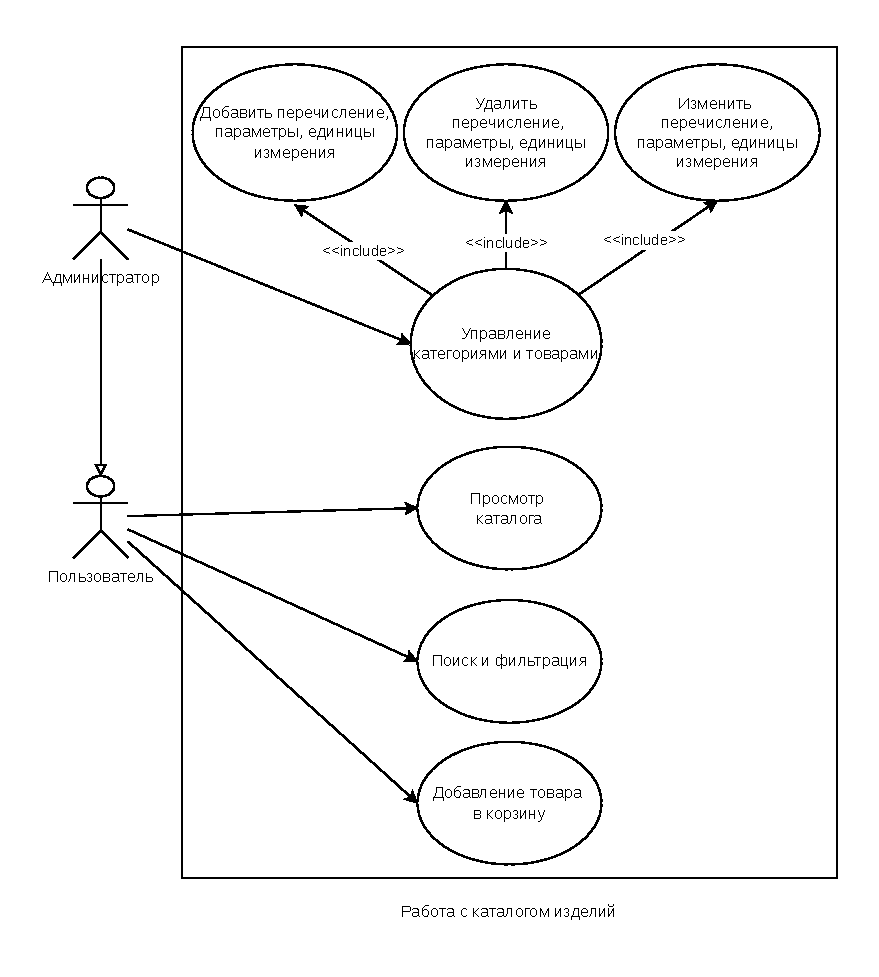
\includegraphics[width=0.95\textwidth]{img/USE-CASE-5.pdf}}
        {\fbox{\parbox{0.9\textwidth}{\centering Место для вставки файла \texttt{img/USE-CASE-5.pdf}}}}
    \caption{Диаграмма вариантов использования}
\end{figure}

Диаграмма отражает разделение функций между обычным пользователем и администратором. Пользовательские сценарии связаны с поиском и выбором товаров, а административные сценарии -- с изменением справочных данных. Такое разделение упрощает интерфейс: пользователь видит только витрину и корзину, а инструменты редактирования вынесены в отдельный административный блок.

\subsection{Разработка приложения}

\subsubsection{Архитектура информационной системы}

Приложение представляет собой модульное монолитное web-приложение. Серверная часть, API, логика работы со справочником и отдача статических файлов находятся в одном Python-приложении. Отдельного frontend-сервера нет: страница интерфейса, стили и JavaScript-файл отдаются тем же FastAPI-приложением, которое обрабатывает REST-запросы.

Точка входа приложения находится в файле \texttt{src/main.py}. При запуске создаётся объект \texttt{FastAPI}, подключаются маршруты API, монтируется директория \texttt{src/static}, а корневой адрес \texttt{/} отдаёт файл \texttt{index.html}. В жизненном цикле приложения также выполняется подготовка базы данных: создаётся база при необходимости, создаются таблицы и закрывается подключение при остановке сервера.

Компоненты системы:
\begin{enumerate}
    \item Серверное приложение на FastAPI. Оно принимает HTTP-запросы, маршрутизирует их и возвращает ответы в формате JSON. Основные маршруты собраны в \texttt{src/api/database.py}; общий роутер подключается через \texttt{src/api/\_\_init\_\_.py}. Для проверки работы сервера и получения общей информации используется отдельный модуль \texttt{src/api/info.py}.
    \item Модели запросов и ответов. В файле \texttt{src/api/models.py} описаны Pydantic-модели для категорий, товаров, спецификаций, параметров, перечислений, единиц измерения и значений параметров. Эти модели проверяют входные данные до передачи их в слой работы с базой.
    \item Слой работы с базой данных. Основная логика находится в \texttt{src/db/database.py}. В этом файле описаны таблицы SQLAlchemy Core, ограничения, связи между таблицами и функции для создания, чтения, изменения и удаления данных. Здесь же реализована проверка бизнес-правил: например, запрет отрицательной цены, проверка значений перечислений и проверка диапазонов числовых параметров.
    \item База данных PostgreSQL. PostgreSQL используется как внешнее хранилище справочника. В базе находятся категории, товары, характеристики, перечисления, значения перечислений, единицы измерения, параметры категорий и значения параметров конкретных товаров.
    \item Статический frontend. Пользовательский интерфейс состоит из файлов \texttt{src/static/index.html}, \texttt{src/static/styles.css} и \texttt{src/static/app.js}. Клиентская часть загружает данные через REST API, отображает витрину, фильтры, корзину и административные формы. Корзина хранится на стороне браузера в \texttt{localStorage}.
    \item Контейнеризация. Для запуска проекта используется \texttt{Dockerfile} и \texttt{docker-compose.yml}. В compose-файле описаны два сервиса: API-приложение и PostgreSQL. API запускается после проверки готовности базы данных.
\end{enumerate}

Таким образом, приложение остаётся монолитным с точки зрения развёртывания, но внутри разделено на понятные модули: входная точка, API, схемы данных, функции работы с БД и статический интерфейс. Такой вариант проще поддерживать в рамках курсовой работы и достаточно хорошо подходит для справочника, где все основные операции связаны с одной базой данных.

\subsubsection{Диаграмма классов}

Диаграмма классов отражает основные классы предметной области и интерфейсные классы web-приложения. Классы предметной области описывают структуру справочника изделий, параметры, перечисления и единицы измерения. Интерфейсные классы соответствуют основным экранам и блокам пользовательского интерфейса: витрине, фильтрам, корзине, форме входа и административным формам.

\begin{figure}[H]
\centering
\resizebox{\textwidth}{!}{%
\begin{tikzpicture}[
    classbox/.style={
        draw,
        rounded corners,
        align=left,
        font=\scriptsize,
        inner sep=4pt,
        text width=4.5cm
    },
    interface/.style={
        draw,
        rounded corners,
        align=left,
        font=\scriptsize,
        inner sep=4pt,
        text width=4.8cm,
        fill=gray!8
    },
    relation/.style={-{Latex[length=2mm]}, thick},
    dependency/.style={-{Latex[length=2mm]}, dashed, thick},
    reltext/.style={font=\scriptsize, fill=white, inner sep=1pt}
]

\node[interface] (ui_catalog) at (0, 7.4) {
\textbf{<<interface>> CatalogView}\\
\texttt{renderCategories()}\\
\texttt{renderProducts()}\\
\texttt{showProductDetails()}\\
\texttt{addToCart()}
};

\node[interface] (ui_filters) at (5.8, 7.4) {
\textbf{<<interface>> FilterPanel}\\
\texttt{readDraftFilters()}\\
\texttt{validateFilters()}\\
\texttt{applyFilters()}\\
\texttt{resetFilters()}
};

\node[interface] (ui_cart) at (11.6, 7.4) {
\textbf{<<interface>> CartView}\\
\texttt{renderCart()}\\
\texttt{addToCart()}\\
\texttt{setCartQuantity()}\\
\texttt{removeFromCart()}\\
\texttt{clearCart()}
};

\node[interface] (ui_auth) at (17.4, 7.4) {
\textbf{<<interface>> AuthForm}\\
\texttt{handleLoginSubmit()}\\
\texttt{handleLogout()}\\
\texttt{renderAuthState()}\\
\texttt{isAdmin()}
};

\node[interface] (ui_admin) at (17.4, 2.9) {
\textbf{<<interface>> AdminForms}\\
\texttt{handleCategorySubmit()}\\
\texttt{handleProductSubmit()}\\
\texttt{editCategory()}\\
\texttt{editProduct()}\\
\texttt{deleteProduct()}
};

\node[classbox] (category) at (0, 2.9) {
\textbf{Category}\\
\texttt{id}\\
\texttt{name}\\
\texttt{parent\_id}\\
\texttt{create/update/move/delete}
};

\node[classbox] (product) at (5.8, 2.9) {
\textbf{Product}\\
\texttt{id}\\
\texttt{name}\\
\texttt{category\_id}\\
\texttt{price}\\
\texttt{quantity}\\
\texttt{specifications}
};

\node[classbox] (specification) at (11.6, 2.9) {
\textbf{Specification}\\
\texttt{id}\\
\texttt{name}\\
\texttt{value}\\
\texttt{enum\_value\_id}\\
\texttt{unit\_id}\\
\texttt{custom unit}
};

\node[classbox] (parameter) at (0, -1.6) {
\textbf{Parameter}\\
\texttt{id}\\
\texttt{code}\\
\texttt{name}\\
\texttt{parameter\_type}\\
\texttt{unit\_id}\\
\texttt{enum\_id}
};

\node[classbox] (category_parameter) at (5.8, -1.6) {
\textbf{CategoryParameter}\\
\texttt{category\_id}\\
\texttt{parameter\_id}\\
\texttt{priority}\\
\texttt{is\_required}\\
\texttt{is\_inherited}\\
\texttt{min/max value}
};

\node[classbox] (product_parameter_value) at (11.6, -1.6) {
\textbf{ProductParameterValue}\\
\texttt{product\_id}\\
\texttt{parameter\_id}\\
\texttt{val\_real}\\
\texttt{val\_int}\\
\texttt{val\_str}\\
\texttt{val\_datetime}\\
\texttt{enum\_value\_id}
};

\node[classbox] (enumeration) at (0, -6.1) {
\textbf{Enumeration}\\
\texttt{id}\\
\texttt{name}\\
\texttt{description}\\
\texttt{created\_at}\\
\texttt{updated\_at}
};

\node[classbox] (enumeration_value) at (5.8, -6.1) {
\textbf{EnumerationValue}\\
\texttt{id}\\
\texttt{enum\_id}\\
\texttt{item\_type}\\
\texttt{value}\\
\texttt{child\_enum\_id}\\
\texttt{priority}
};

\node[classbox] (unit) at (11.6, -6.1) {
\textbf{MeasurementUnit}\\
\texttt{id}\\
\texttt{full\_name}\\
\texttt{short\_name}\\
\texttt{description}
};

\draw[dependency] (ui_catalog) -- node[reltext, left]{shows} (category);
\draw[dependency] (ui_catalog) -- node[reltext, left]{shows} (product);
\draw[dependency] (ui_filters) -- node[reltext, left]{filters} (product);
\draw[dependency] (ui_filters) -- node[reltext, right]{by specs} (specification);
\draw[dependency] (ui_cart) -- node[reltext, right]{contains} (product);
\draw[dependency] (ui_auth) -- node[reltext, right]{opens access} (ui_admin);
\draw[dependency] (ui_admin) -- node[reltext, above]{edits} (category);
\draw[dependency] (ui_admin) -- node[reltext, right]{edits} (product);

\draw[relation] (category) -- node[reltext, above]{1:N} (product);
\draw[relation] (product) -- node[reltext, above]{N:M} (specification);
\draw[relation] (category) -- node[reltext, above]{1:N} (category_parameter);
\draw[relation] (parameter) -- node[reltext, above]{1:N} (category_parameter);
\draw[relation] (product) -- node[reltext, above]{1:N} (product_parameter_value);
\draw[relation] (parameter) -- node[reltext, above]{1:N} (product_parameter_value);
\draw[relation] (enumeration) -- node[reltext, above]{1:N} (enumeration_value);
\draw[relation] (enumeration) to[bend right=18] node[reltext, below]{nested enum} (enumeration_value);
\draw[relation] (enumeration) -- node[reltext, left]{type} (parameter);
\draw[relation] (unit) -- node[reltext, right]{unit} (parameter);
\draw[relation] (unit) -- node[reltext, right]{unit} (specification);
\draw[relation] (enumeration_value) -- node[reltext, right]{enum value} (specification);
\draw[relation] (enumeration_value) -- node[reltext, above]{enum value} (product_parameter_value);

\end{tikzpicture}%
}
\caption{Диаграмма классов приложения}
\end{figure}

На диаграмме показано, что центральным классом справочника является \texttt{Product}, который относится к категории, имеет набор характеристик и значения настраиваемых параметров. Классы \texttt{Enumeration}, \texttt{EnumerationValue} и \texttt{MeasurementUnit} используются как вспомогательные справочники для параметров и характеристик. Интерфейсные классы отделены от предметных классов пунктирными зависимостями: они не хранят данные самостоятельно, а отображают их пользователю и вызывают операции чтения или изменения через API.

\subsubsection{ERD диаграмма}

ERD диаграмма построена по фактической структуре таблиц, описанной в модуле \texttt{src/db/database.py}. В модели выделены сущности для дерева категорий, товаров, характеристик, параметров, перечислений, единиц измерения и таблиц связей, которые позволяют назначать параметры категориям и хранить значения параметров конкретных товаров.

\begin{figure}[H]
\centering
\resizebox{\textwidth}{!}{%
\begin{tikzpicture}[
    entity/.style={
        draw,
        rounded corners,
        align=left,
        font=\scriptsize,
        inner sep=4pt,
        text width=4.2cm
    },
    relation/.style={-{Latex[length=2mm]}, thick},
    optional/.style={-{Latex[length=2mm]}, dashed, thick},
    reltext/.style={font=\scriptsize, fill=white, inner sep=1pt}
]

\node[entity] (categories) at (0, 8) {
\textbf{categories}\\
\texttt{id} PK\\
\texttt{name}\\
\texttt{parent\_id} FK categories.id\\
UNIQUE(\texttt{parent\_id}, \texttt{name})
};

\node[entity] (products) at (6, 8) {
\textbf{products}\\
\texttt{id} PK\\
\texttt{name}\\
\texttt{category\_id} FK categories.id\\
\texttt{price}\\
\texttt{quantity}\\
\texttt{description}
};

\node[entity] (product_specifications) at (12, 8) {
\textbf{product\_specifications}\\
\texttt{product\_id} PK, FK products.id\\
\texttt{specification\_id} PK, FK specifications.id
};

\node[entity] (specifications) at (18, 8) {
\textbf{specifications}\\
\texttt{id} PK\\
\texttt{name}\\
\texttt{value}\\
\texttt{enum\_value\_id} FK enumeration\_values.id\\
\texttt{unit\_id} FK measurement\_units.id\\
\texttt{custom\_unit\_full\_name}\\
\texttt{custom\_unit\_short\_name}
};

\node[entity] (category_parameters) at (0, 3.5) {
\textbf{category\_parameters}\\
\texttt{id} PK\\
\texttt{category\_id} FK categories.id\\
\texttt{parameter\_id} FK parameters.id\\
\texttt{source\_category\_id} FK categories.id\\
\texttt{priority}\\
\texttt{is\_required}\\
\texttt{is\_inherited}\\
\texttt{min\_value}\\
\texttt{max\_value}
};

\node[entity] (parameters) at (6, 3.5) {
\textbf{parameters}\\
\texttt{id} PK\\
\texttt{code} UNIQUE\\
\texttt{name}\\
\texttt{description}\\
\texttt{parameter\_type}\\
\texttt{unit\_id} FK measurement\_units.id\\
\texttt{enum\_id} FK enumerations.id
};

\node[entity] (product_parameter_values) at (12, 3.5) {
\textbf{product\_parameter\_values}\\
\texttt{id} PK\\
\texttt{product\_id} FK products.id\\
\texttt{parameter\_id} FK parameters.id\\
\texttt{val\_real}\\
\texttt{val\_int}\\
\texttt{val\_str}\\
\texttt{val\_datetime}\\
\texttt{enum\_value\_id} FK enumeration\_values.id
};

\node[entity] (measurement_units) at (0, -1.3) {
\textbf{measurement\_units}\\
\texttt{id} PK\\
\texttt{full\_name} UNIQUE\\
\texttt{short\_name} UNIQUE\\
\texttt{description}
};

\node[entity] (enumerations) at (6, -1.3) {
\textbf{enumerations}\\
\texttt{id} PK\\
\texttt{name} UNIQUE\\
\texttt{description}\\
\texttt{created\_at}\\
\texttt{updated\_at}
};

\node[entity] (enumeration_values) at (12, -1.3) {
\textbf{enumeration\_values}\\
\texttt{id} PK\\
\texttt{enum\_id} FK enumerations.id\\
\texttt{item\_type}\\
\texttt{value}\\
\texttt{child\_enum\_id} FK enumerations.id\\
\texttt{priority}\\
\texttt{description}
};

\draw[relation] (categories) -- node[reltext, above]{1:N} (products);
\draw[relation] (categories) -- node[reltext, left]{1:N} (category_parameters);
\draw[optional] (categories.south east) to[bend right=20] node[reltext, right]{source} (category_parameters.north east);
\draw[relation] (products) -- node[reltext, above]{1:N} (product_specifications);
\draw[relation] (specifications) -- node[reltext, above]{1:N} (product_specifications);
\draw[relation] (products.south) to[bend left=15] node[reltext, right]{1:N} (product_parameter_values.north);
\draw[relation] (parameters) -- node[reltext, above]{1:N} (category_parameters);
\draw[relation] (parameters) -- node[reltext, above]{1:N} (product_parameter_values);
\draw[relation] (measurement_units) -- node[reltext, left]{1:N} (parameters);
\draw[relation]
    (measurement_units.south) -- ++(0,-1.0) -| node[reltext, pos=0.75, above]{1:N} (specifications.south);
\draw[relation] (enumerations) -- node[reltext, above]{1:N} (enumeration_values);
\draw[relation] (enumerations.north east) to[bend left=20] node[reltext, right]{child enum} (enumeration_values.north west);
\draw[relation] (enumerations) -- node[reltext, right]{1:N} (parameters);
\draw[relation] (enumeration_values) -- node[reltext, right]{1:N} (product_parameter_values);
\draw[relation] (enumeration_values.north east) to[bend right=15] node[reltext, right]{1:N} (specifications.south);

\end{tikzpicture}%
}
\caption{ERD диаграмма базы данных приложения}
\end{figure}

На диаграмме сплошные линии показывают основные внешние ключи, а пунктирная связь используется для указания исходной категории при наследовании параметров. Таблица \texttt{enumeration\_values} хранит как конечные значения перечислений, так и ссылки на вложенные перечисления через поле \texttt{child\_enum\_id}, поэтому она связана с таблицей \texttt{enumerations} двумя внешними ключами.

Основные таблицы проекта:
\begin{itemize}
    \item \texttt{categories} -- дерево категорий справочника;
    \item \texttt{products} -- товары, привязанные к категориям;
    \item \texttt{specifications} -- характеристики товаров;
    \item \texttt{product\_specifications} -- связь товаров с характеристиками;
    \item \texttt{measurement\_units} -- справочник единиц измерения;
    \item \texttt{enumerations} -- справочник перечислений;
    \item \texttt{enumeration\_values} -- значения перечислений и вложенные перечисления;
    \item \texttt{parameters} -- метаданные параметров;
    \item \texttt{category\_parameters} -- параметры, назначенные категориям;
    \item \texttt{product\_parameter\_values} -- значения параметров конкретных товаров.
\end{itemize}

\subsubsection{Технологии разработки}

Для разработки серверной части выбран FastAPI, так как он позволяет быстро создавать REST API, автоматически формирует Swagger-документацию и поддерживает асинхронную работу. Для хранения данных используется PostgreSQL. Работа с базой данных выполняется через SQLAlchemy Core.

Пользовательский интерфейс реализован без отдельного frontend-фреймворка: HTML, CSS и JavaScript отдаются самим FastAPI-приложением. Такой подход упрощает запуск проекта и соответствует формату курсовой работы.

Использованные технологии:
\begin{itemize}
    \item Python;
    \item FastAPI;
    \item PostgreSQL;
    \item SQLAlchemy Core;
    \item HTML;
    \item CSS;
    \item JavaScript;
    \item Docker.
\end{itemize}

\subsubsection{Тестирование приложения}

Функциональное тестирование проводилось вручную по основным сценариям использования web-приложения и REST API. Проверялись публичные функции витрины, работа корзины, авторизация администратора и операции изменения справочных данных. Ниже приведены тестовые сценарии и места для скриншотов, подтверждающих выполнение проверок.

\begin{enumerate}
    \item Авторизация и разграничение прав.

    Сценарий: пользователь открывает сайт без авторизации и просматривает витрину товаров. Затем выполняется вход под учетной записью администратора через форму в административном разделе.

    Ожидаемый результат: без авторизации доступны каталог, витрина, фильтры и корзина, но кнопки редактирования и формы управления скрыты. После входа администратора отображаются формы создания категорий и товаров, а на карточках появляются кнопки изменения и удаления.

    \begin{figure}[H]
        \centering
        \IfFileExists{img/test-auth-user.png}
            {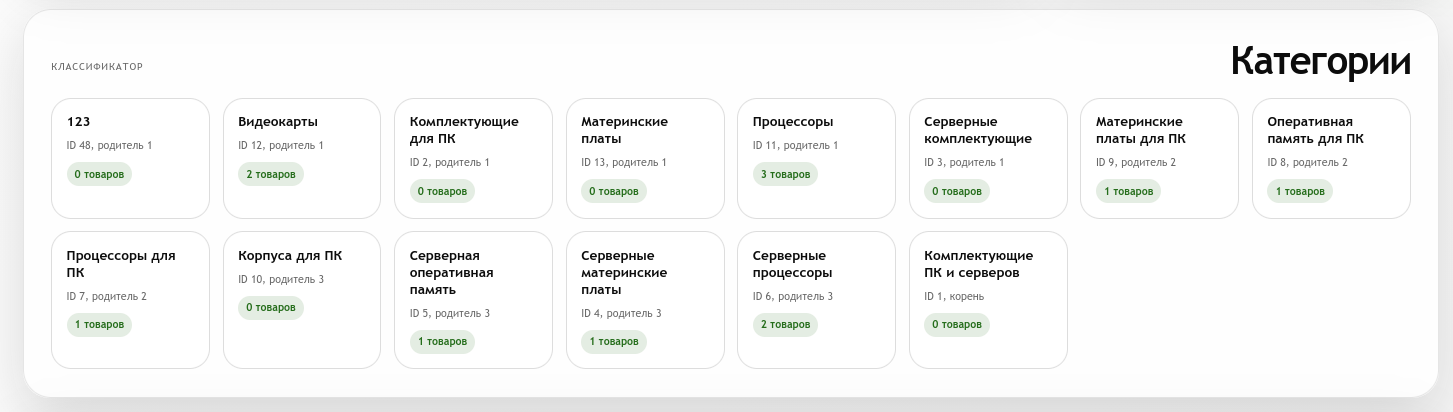
\includegraphics[width=0.9\textwidth]{img/test-auth-user.png}}
            {\fbox{\parbox{0.85\textwidth}{\centering Место для скриншота режима просмотра без авторизации}}}
        \caption{Витрина в режиме просмотра}
    \end{figure}

    \begin{figure}[H]
        \centering
        \IfFileExists{img/test-auth-admin.png}
            {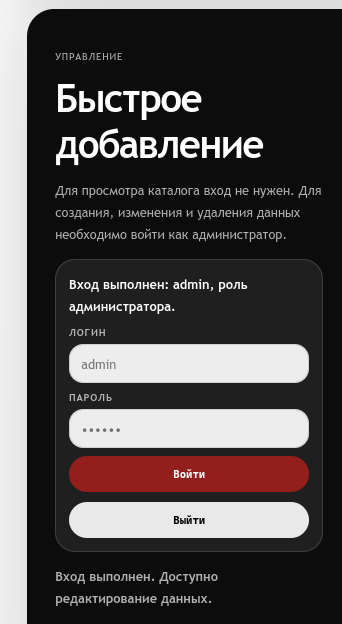
\includegraphics[width=0.5\textwidth]{img/test-auth-admin.png}}
            {\fbox{\parbox{0.85\textwidth}{\centering Место для скриншота входа администратора}}}
        \caption{Вход администратора}
    \end{figure}

    \begin{figure}[H]
        \centering
        \IfFileExists{img/test-auth-admin-cat.png}
            {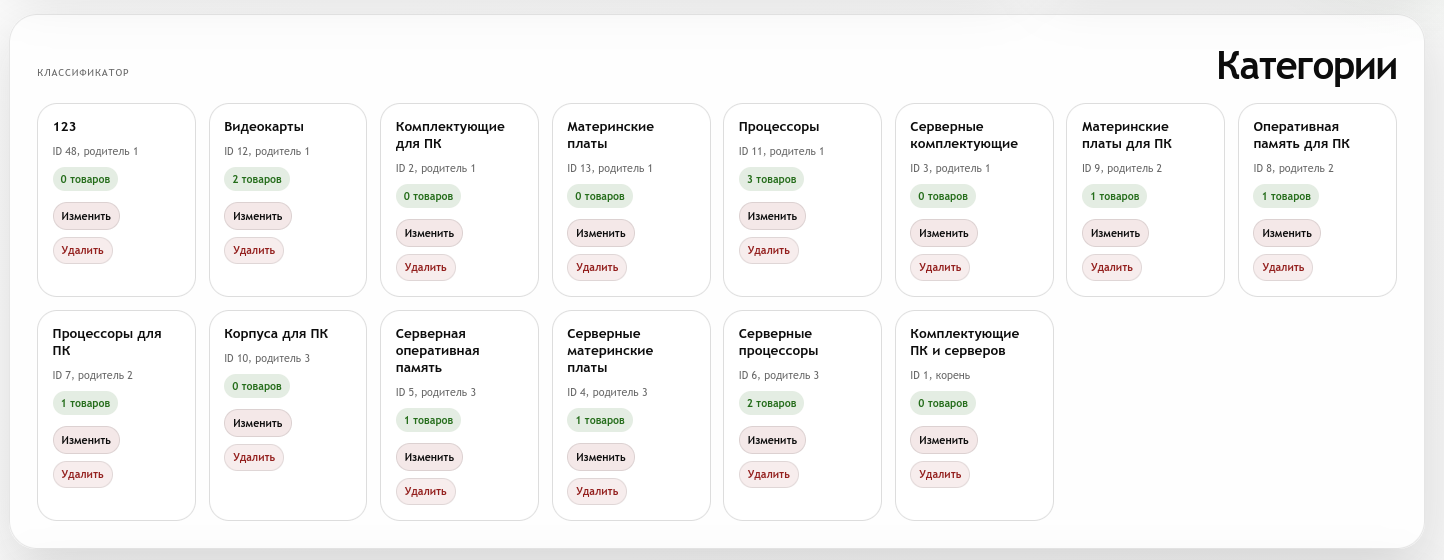
\includegraphics[width=0.9\textwidth]{img/test-auth-admin-cat.png}}
            {\fbox{\parbox{0.85\textwidth}{\centering Место для скриншота входа администратора}}}
        \caption{Отображение форм управления}
    \end{figure}

    \item Создание категории.

    Сценарий: администратор переходит в административный блок, заполняет название новой категории, выбирает родительский раздел и нажимает кнопку создания.

    Ожидаемый результат: новая категория сохраняется в базе данных, появляется в списке категорий и становится доступной в выпадающем списке фильтра по категории.

    \begin{figure}[H]
        \centering
        \IfFileExists{img/test-auth-admin-cat.png}
            {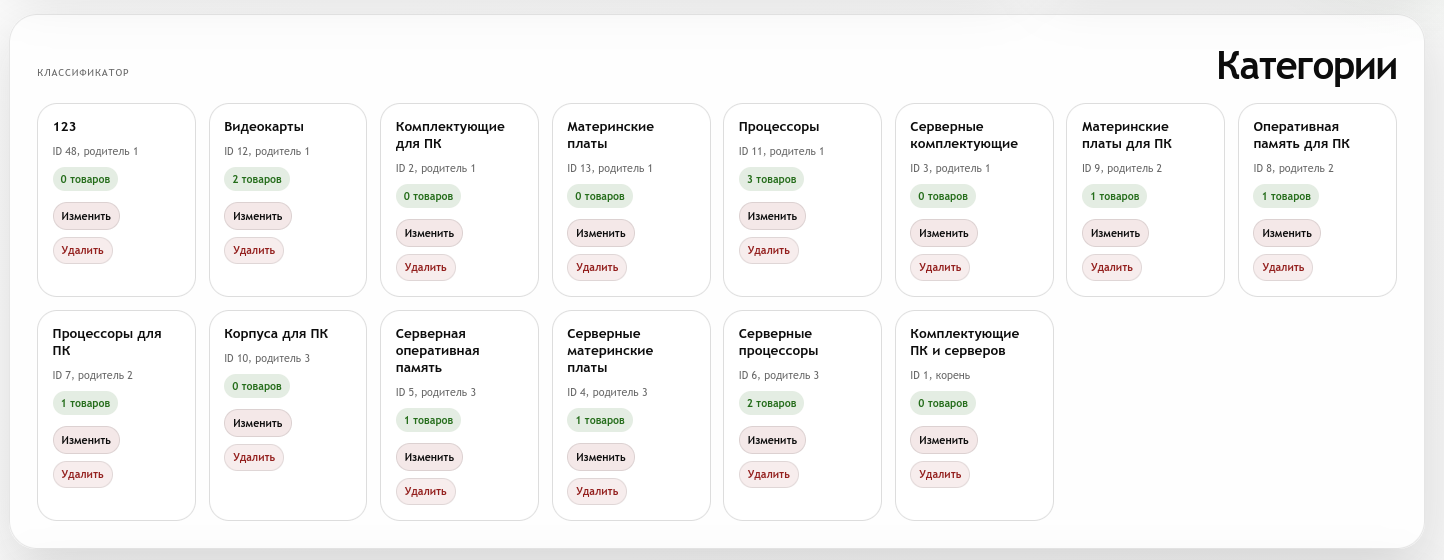
\includegraphics[width=0.9\textwidth]{img/test-auth-admin-cat.png}}
            {\fbox{\parbox{0.85\textwidth}{\centering Место для скриншота входа администратора}}}
        \caption{Отображение форм управления до создания категории}
    \end{figure}

    \begin{figure}[H]
        \centering
        \IfFileExists{img/test-category-create.png}
            {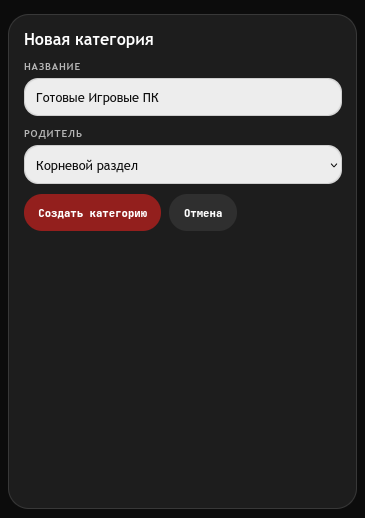
\includegraphics[width=0.9\textwidth]{img/test-category-create.png}}
            {\fbox{\parbox{0.85\textwidth}{\centering Место для скриншота формы создания категории}}}
        \caption{Создание категории}
    \end{figure}

    \begin{figure}[H]
        \centering
        \IfFileExists{img/test-category-result.png}
            {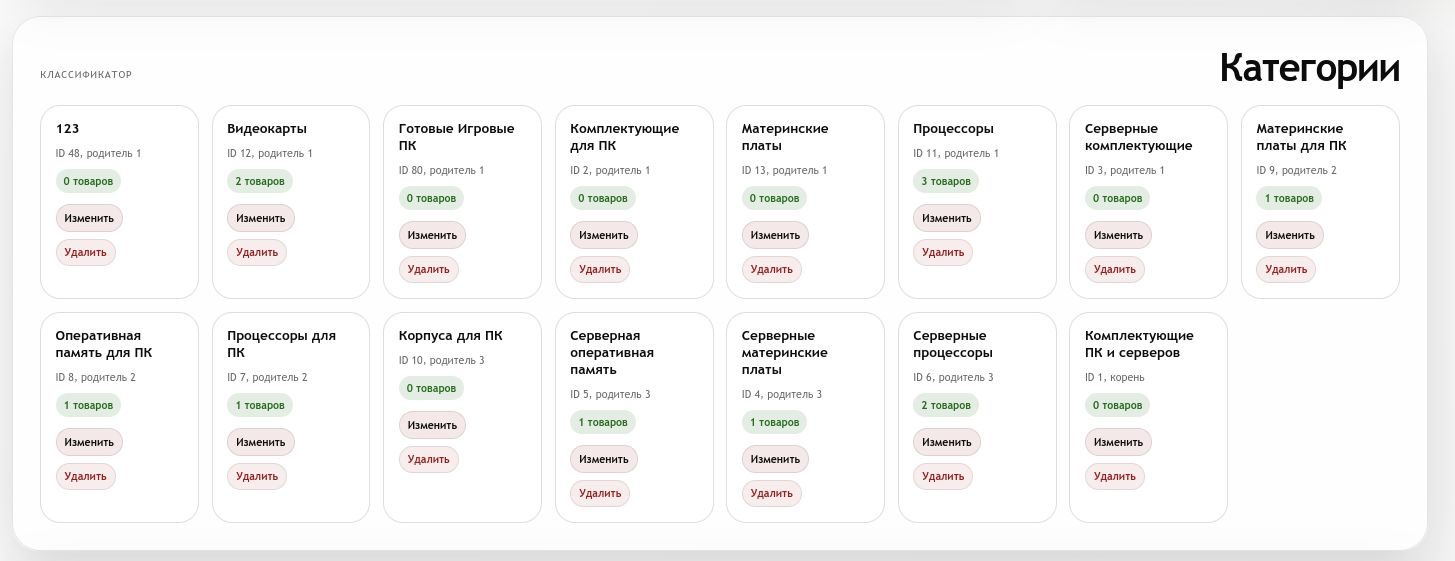
\includegraphics[width=0.9\textwidth]{img/test-category-result.png}}
            {\fbox{\parbox{0.85\textwidth}{\centering Место для скриншота обновленного списка категорий}}}
        \caption{Категория добавлена в классификатор}
    \end{figure}

    \item Создание товара с характеристиками.

    Сценарий: администратор заполняет форму нового товара, указывает категорию, цену, остаток и описание. После сохранения товар добавляется в справочник и отображается на витрине.

    Ожидаемый результат: товар создается через защищенный endpoint, появляется в карточках витрины, а его цена, остаток, категория и описание отображаются корректно.

    \begin{figure}[H]
        \centering
        \IfFileExists{img/test-product-create.png}
            {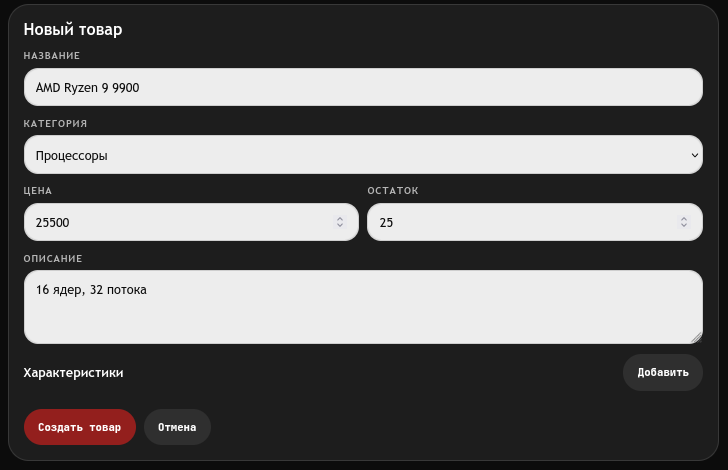
\includegraphics[width=0.9\textwidth]{img/test-product-create.png}}
            {\fbox{\parbox{0.85\textwidth}{\centering Место для скриншота формы создания товара}}}
        \caption{Создание товара}
    \end{figure}

    \begin{figure}[H]
        \centering
        \IfFileExists{img/test-product-result.png}
            {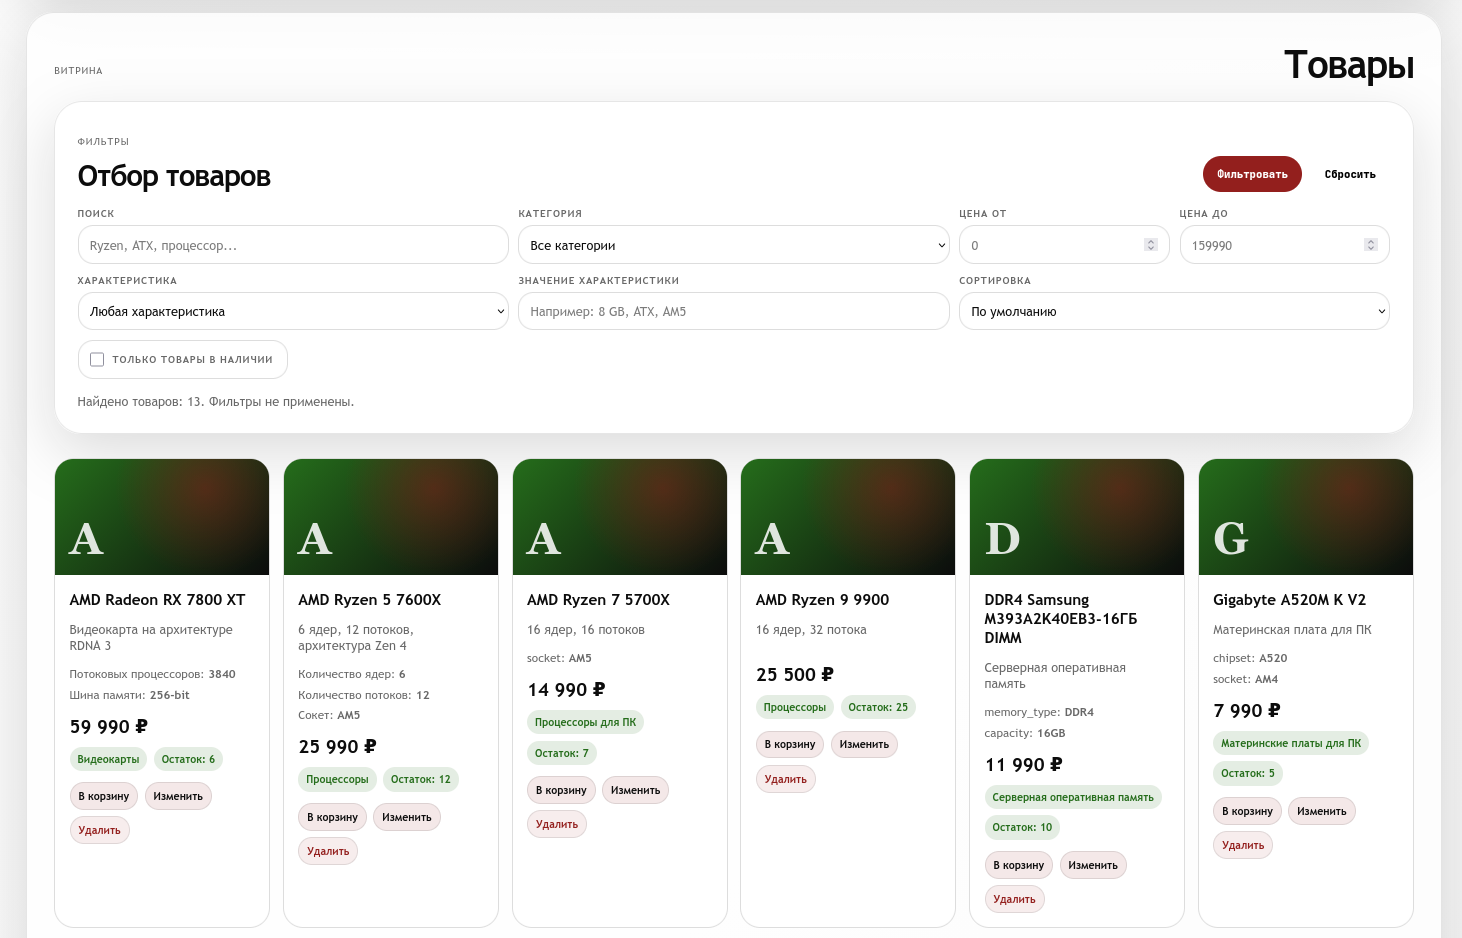
\includegraphics[width=0.9\textwidth]{img/test-product-result.png}}
            {\fbox{\parbox{0.85\textwidth}{\centering Место для скриншота товара на витрине}}}
        \caption{Новый товар на витрине}
    \end{figure}

    \item Управление перечислениями.

    Сценарий: администратор создает перечисление, например «Сокеты процессоров», и добавляет значения AM4, AM5 и LGA1700. Затем значение перечисления используется в характеристике товара.

    Ожидаемый результат: перечисление и его значения сохраняются в таблицах \texttt{enumerations} и \texttt{enumeration\_values}. На витрине характеристика отображается названием значения, например AM5, а не техническим идентификатором.

    \begin{figure}[H]
        \centering
        \IfFileExists{img/test-enum-create.png}
            {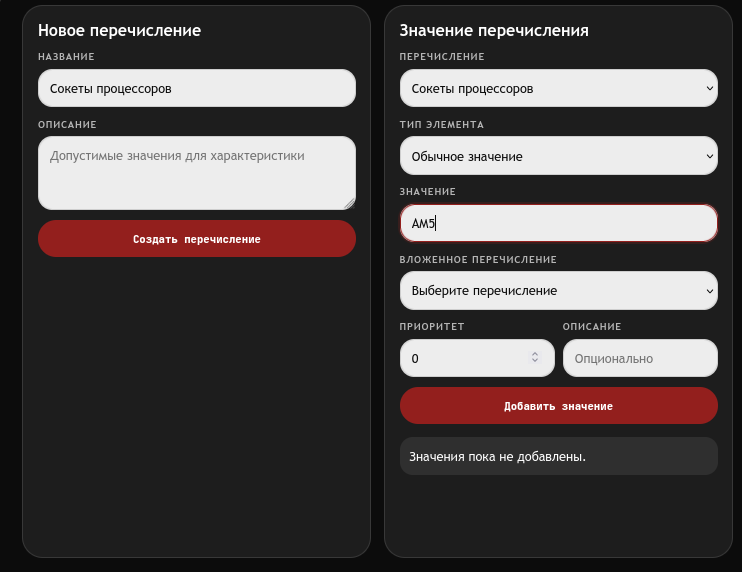
\includegraphics[width=0.9\textwidth]{img/test-enum-create.png}}
            {\fbox{\parbox{0.85\textwidth}{\centering Место для скриншота создания перечисления в Swagger}}}
        \caption{Создание перечисления и его значений}
    \end{figure}

    \begin{figure}[H]
        \centering
        \IfFileExists{img/test-enum-value-display.png}
            {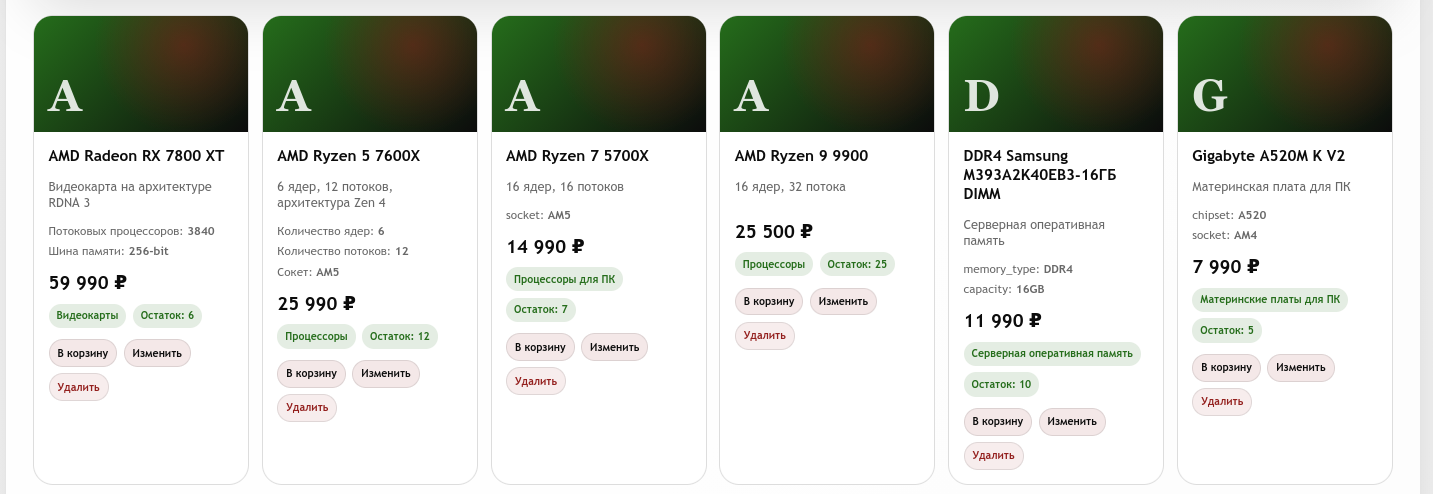
\includegraphics[width=0.9\textwidth]{img/test-enum-value-display.png}}
            {\fbox{\parbox{0.85\textwidth}{\centering Место для скриншота отображения значения перечисления на витрине}}}
        \caption{Отображение значения перечисления в характеристиках товара}
    \end{figure}

    % \item Настройка параметров категории и запись значения параметра товара.

    % Сценарий: администратор создает параметр, назначает его категории с ограничениями минимального и максимального значения, затем записывает значение параметра для конкретного товара.

    % Ожидаемый результат: параметр появляется в списке параметров категории, значение товара сохраняется в таблице \texttt{product\_parameter\_values}. При нарушении заданного диапазона API возвращает ошибку валидации.

    % \begin{figure}[H]
    %     \centering
    %     \IfFileExists{img/test-parameter-assign.png}
    %         {\includegraphics[width=0.9\textwidth]{img/test-parameter-assign.png}}
    %         {\fbox{\parbox{0.85\textwidth}{\centering Место для скриншота назначения параметра категории}}}
    %     \caption{Назначение параметра категории}
    % \end{figure}

    % \begin{figure}[H]
    %     \centering
    %     \IfFileExists{img/test-parameter-value.png}
    %         {\includegraphics[width=0.9\textwidth]{img/test-parameter-value.png}}
    %         {\fbox{\parbox{0.85\textwidth}{\centering Место для скриншота записи значения параметра товара}}}
    %     \caption{Запись значения параметра товара}
    % \end{figure}

    \item Поиск и фильтрация товаров на витрине.

    Сценарий: пользователь задает фильтры на витрине: категорию, диапазон цены, наличие на складе, характеристику и значение характеристики. После нажатия кнопки «Фильтровать» выполняется проверка введенных данных.

    Ожидаемый результат: при корректных значениях витрина показывает только подходящие товары. При некорректном диапазоне, например отрицательной цене или нижней границе больше верхней, появляется всплывающее сообщение, а фильтрация не выполняется.

    \begin{figure}[H]
        \centering
        \IfFileExists{img/test-filters-result.png}
            {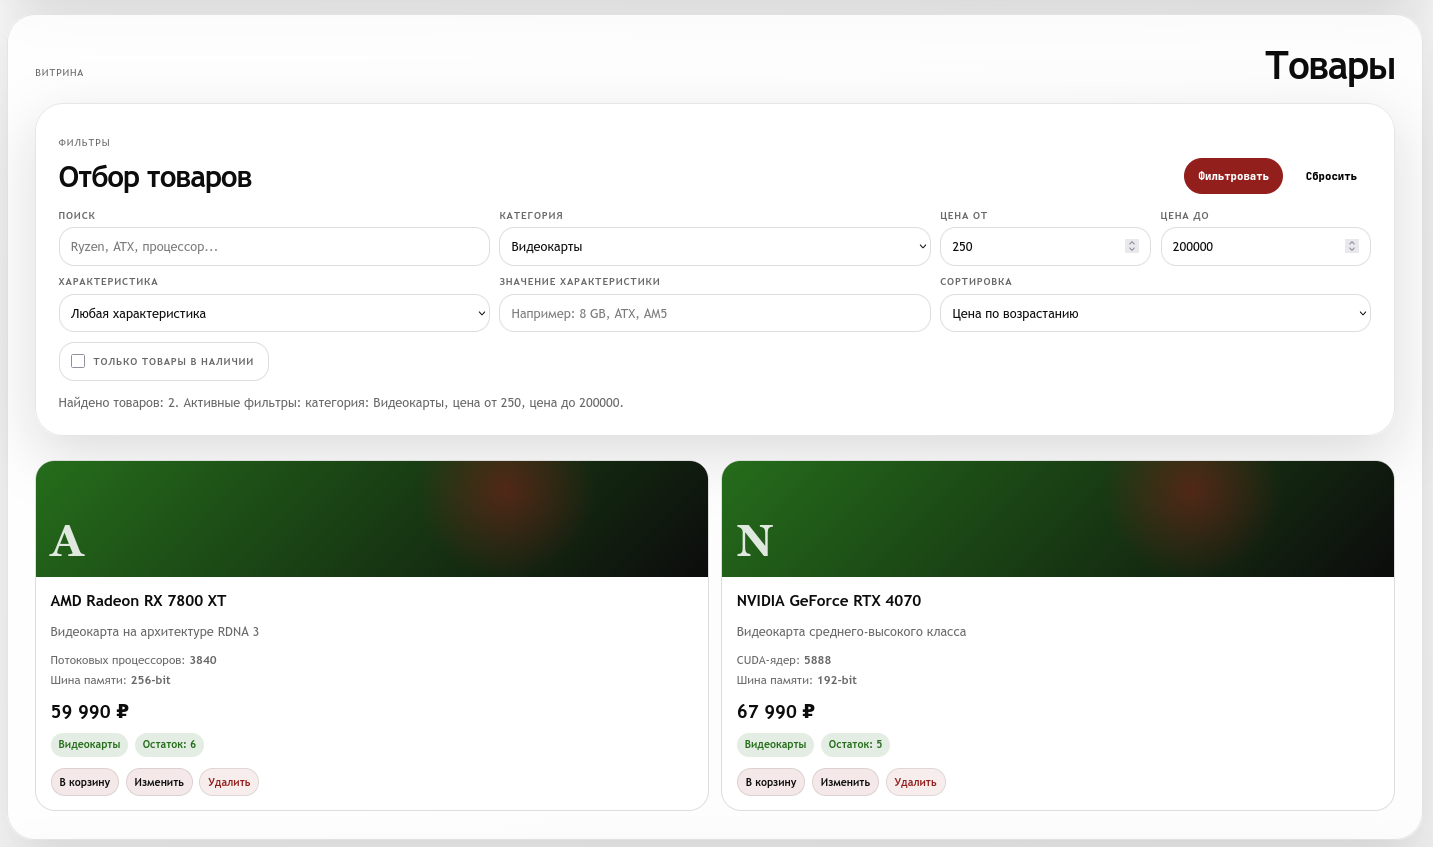
\includegraphics[width=0.9\textwidth]{img/test-filters-result.png}}
            {\fbox{\parbox{0.85\textwidth}{\centering Место для скриншота результата фильтрации товаров}}}
        \caption{Результат фильтрации товаров}
    \end{figure}

    \begin{figure}[H]
        \centering
        \IfFileExists{img/test-filters-validation.png}
            {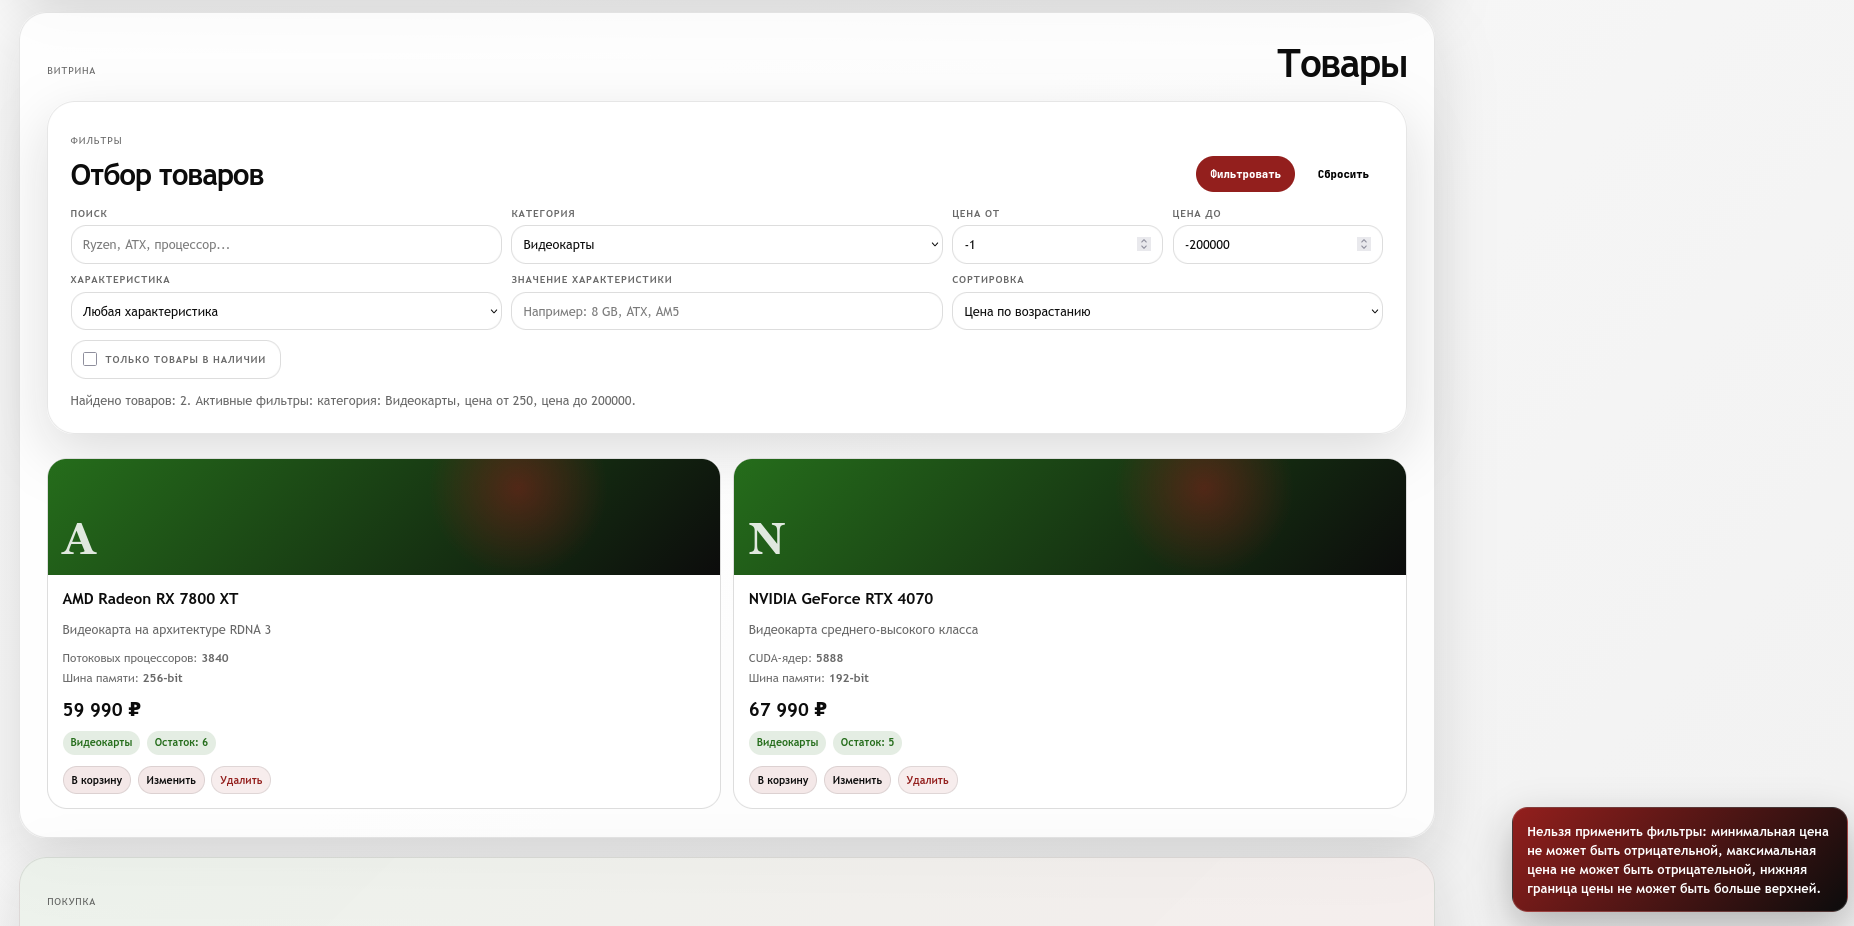
\includegraphics[width=0.9\textwidth]{img/test-filters-validation.png}}
            {\fbox{\parbox{0.85\textwidth}{\centering Место для скриншота ошибки валидации фильтров}}}
        \caption{Ошибка валидации фильтров}
    \end{figure}

    \item Работа с корзиной.

    Сценарий: пользователь добавляет товар в корзину, изменяет количество, удаляет одну позицию и очищает корзину. Затем нажимает кнопку «Заказать».

    Ожидаемый результат: количество товаров и итоговая сумма пересчитываются на стороне клиента. При нажатии кнопки «Заказать» выводится уведомление о том, что оформление заказа пока не реализовано.

    \begin{figure}[H]
        \centering
        \IfFileExists{img/test-cart.png}
            {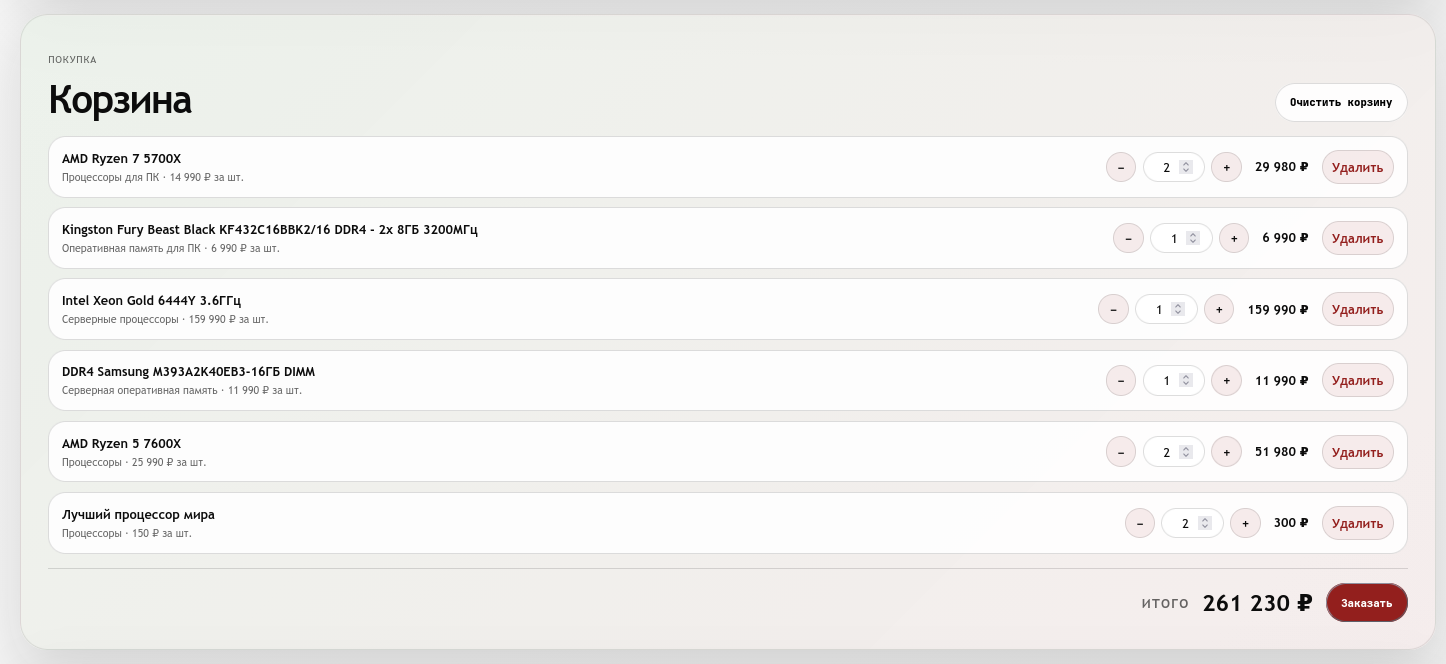
\includegraphics[width=0.9\textwidth]{img/test-cart.png}}
            {\fbox{\parbox{0.85\textwidth}{\centering Место для скриншота корзины с товарами}}}
        \caption{Корзина с добавленными товарами}
    \end{figure}

    \begin{figure}[H]
        \centering
        \IfFileExists{img/test-cart-order.png}
            {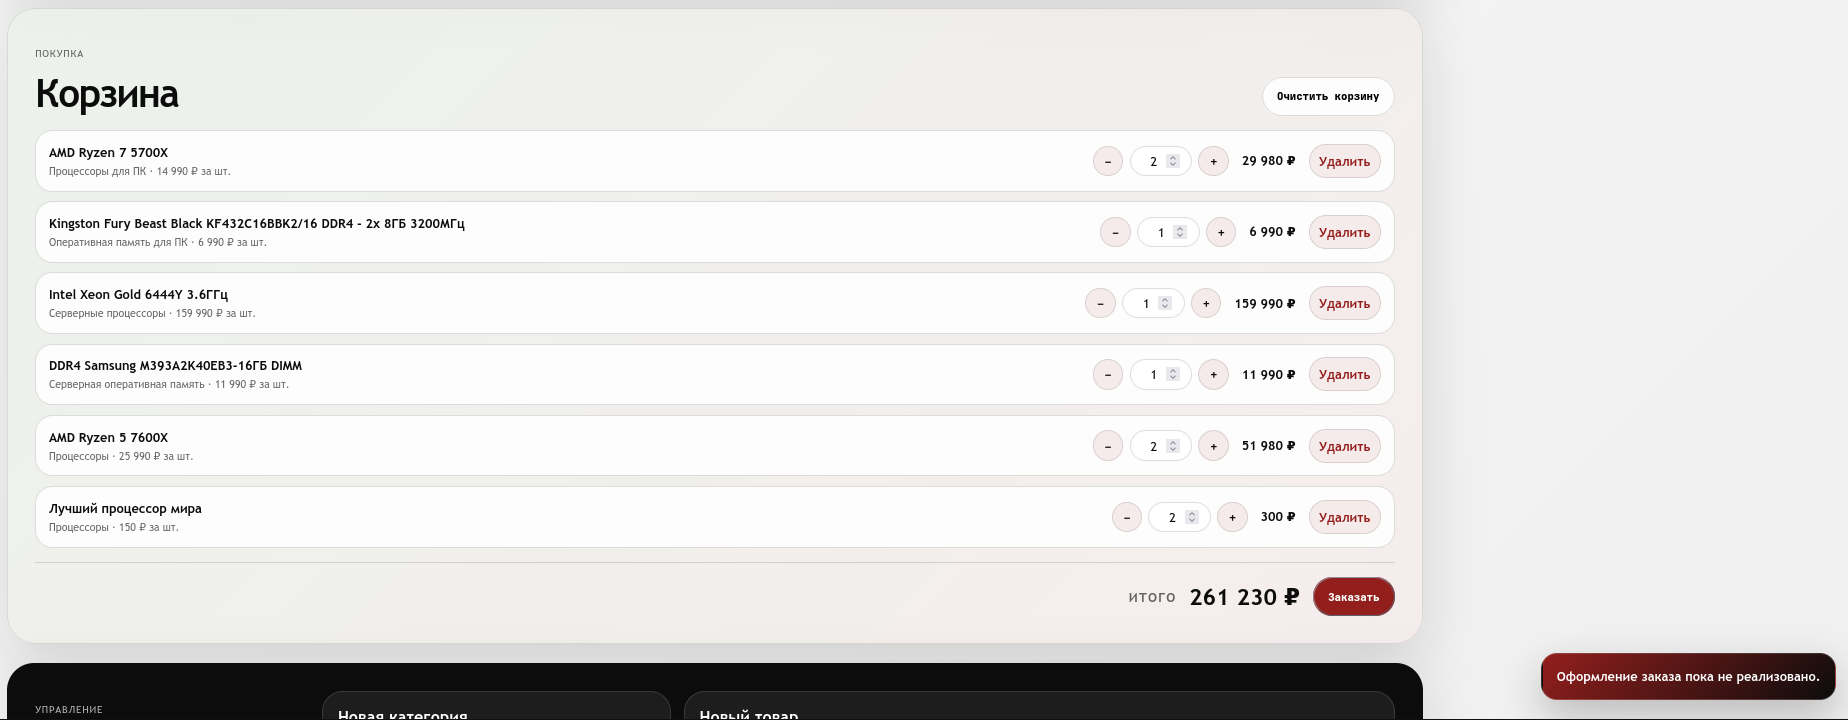
\includegraphics[width=0.9\textwidth]{img/test-cart-order.png}}
            {\fbox{\parbox{0.85\textwidth}{\centering Место для скриншота уведомления при заказе}}}
        \caption{Уведомление при попытке оформления заказа}
    \end{figure}

Все описанные сценарии завершились успешно. Публичные операции чтения доступны пользователю без авторизации, а операции создания, редактирования и удаления выполняются только после входа администратора. Ошибки валидации отображаются пользователю в виде понятных сообщений, а серверные ограничения предотвращают запись некорректных данных в базу.

\subsection{Разработка пользовательского интерфейса}

\subsubsection{Информационная архитектура}

Информационная архитектура web-интерфейса включает следующие основные разделы:
\begin{itemize}
    \item главная страница;
    \item каталог категорий;
    \item витрина товаров;
    \item фильтры товаров;
    \item корзина;
    \item административный блок;
    \item Swagger API.
\end{itemize}

Навигация на desktop-устройствах расположена в верхней части страницы. Для мобильных устройств реализована нижняя панель навигации с основными действиями.

\subsubsection{Диаграмма потоков задач}

В данном разделе необходимо вставить Task Flow диаграмму.

Основные пользовательские потоки:
\begin{itemize}
    \item просмотр категории → выбор фильтров → фильтрация → просмотр товара;
    \item просмотр товара → добавление в корзину → изменение количества → оформление заказа;
    \item администратор → создание категории → создание товара → проверка товара на витрине;
    \item администратор → создание перечисления → добавление значения → использование значения в характеристике.
\end{itemize}

\subsubsection{Выбор цветов и шрифтов}

Для интерфейса выбрана контрастная цветовая палитра:
\begin{itemize}
    \item \texttt{\#931F1D} -- акцентный цвет для основных кнопок и уведомлений;
    \item \texttt{\#256D1B} -- дополнительный зелёный цвет для меток и элементов состояния;
    \item \texttt{\#0C0C0C} -- основной тёмный цвет текста и контрастных блоков;
    \item \texttt{\#FFFFFF} -- базовый цвет поверхностей и фона.
\end{itemize}

Выбор палитры связан с необходимостью обеспечить контрастность интерфейса и визуально выделить ключевые действия пользователя. Основной шрифт интерфейса -- sans-serif, для крупных заголовков используется serif-шрифт, что делает главную страницу более выразительной.

\subsubsection{Страницы интерфейса}

В данном разделе необходимо привести скриншоты разработанных страниц и элементов интерфейса.

Реализованные элементы:
\begin{itemize}
    \item главная страница с краткой статистикой;
    \item каталог категорий;
    \item витрина товаров;
    \item фильтры товаров с валидацией;
    \item карточка товара;
    \item корзина;
    \item административные формы добавления и редактирования категорий и товаров;
    \item всплывающие уведомления.
\end{itemize}

\section{Заключение}

В ходе курсовой работы было разработано web-приложение для работы со справочником электронных комплектующих. Была реализована серверная часть, база данных, API и пользовательский интерфейс. Система поддерживает работу с категориями, товарами, характеристиками, перечислениями, единицами измерения, параметрами и корзиной.

В данном разделе необходимо дополнить выводы о выполненных задачах, достигнутых результатах и возможных направлениях развития проекта.

\newpage
\begin{thebibliography}{9}
\bibitem{fastapi} FastAPI Documentation [Электронный ресурс]. URL: \url{https://fastapi.tiangolo.com/}
\bibitem{postgresql} PostgreSQL Documentation [Электронный ресурс]. URL: \url{https://www.postgresql.org/docs/}
\bibitem{sqlalchemy} SQLAlchemy Documentation [Электронный ресурс]. URL: \url{https://docs.sqlalchemy.org/}
\bibitem{wcag} Web Content Accessibility Guidelines (WCAG) 2.1 [Электронный ресурс]. URL: \url{https://www.w3.org/TR/WCAG21/}
\bibitem{iso9241} ГОСТ Р ИСО 9241-161-2016. Эргономика взаимодействия человек-система. Элементы графического пользовательского интерфейса.
\end{thebibliography}

\newpage
\appendix
\section{Приложение А. Скриншоты интерфейса}

В приложение необходимо добавить скриншоты главной страницы, витрины, фильтров, корзины и административных форм.

\section{Приложение Б. Фрагменты программного кода}

В приложение при необходимости можно добавить фрагменты SQL-процедур, API-обработчиков и JavaScript-кода пользовательского интерфейса.

\end{document}
